\chapauthor{Голенков В.В.\\Банцевич К.А.}
\chapter{Структура баз знаний интеллектуальных компьютерных систем нового поколения: иерархическая система предметных областей и соответствующих им онтологий}
\chapauthortoc{Голенков В.В.\\Банцевич К.А.}
\label{chapter_kb}

\abstract{В настоящее время всё более актуальным становится использование интеллектуальных систем в различных областях, что, в свою очередь, требует от данных систем поддержки решения комплексных задач. Ключевым компонентом таких систем является база знаний, которая должна обеспечивать совместное использование различных видов знаний и моделей их представления.}

Основным факторами, определяющими качество интеллектуальной компьютерной системы, являются:
	\begin{itemize}
		\item {качественная структуризация (систематизация) и \uline{стратификация} базы знаний интеллектуальной 		компьютерной системы, а также}
		\item {систематизация и стратификация деятельности, которая осуществляется интеллектуальной компьютерной системой и спецификация которой является важнейшей частью базы знаний этой системы.}
	\end{itemize}

Качественная структуризация базы знаний позволит обеспечить совместимость различных видов знаний, используемых интеллектуальными системами.  

На сегодняшний день наиболее эффективным средством структуризации различных областей знаний являются онтологии. Суть онтологического подхода при проектировании базы знаний заключается в рассмотрении структуры базы знаний как иерархической системы выделенных предметных областей и соответствующих им онтологий. Однако, онтологически существует множество способов, которыми можно описать реальный мир таким, каким он есть. Следовательно, задача обеспечения совместимости различных видов знаний остается актуальной. Решением данной задачи является использование при проектировании баз знаний онтологий верхнего уровня.

\begin{SCn}
	\scnheader{онтология верхнего уровня}
	\scnsuperset{онтология}
	\scnidtf{онтология, описывающая фундаментальные понятия, которые являются общими для всех предметных областей}
	\scnidtf{онтология, систематизирующая знания о реальном мире безотносительно к какой-либо конкретной предметной области}
	\scntext{цель}{поддержка семантической совместимости онтологий предметных областей и прикладных онтологий}	
\end{SCn}

Грамотно построенная онтология верхнего уровня позволит обеспечить широкую семантическую совместимость между большим количеством онтологий для различных предметных областей. Поскольку термины предметно-ориентированных онтологий подчинены терминам онтологии более высокого уровня.

На сегодняшний момент существует несколько разработанных онтологий верхнего уровня:
\begin{itemize}
	\item{\textbf{The Standard Upper Ontology} (SUMO). Назначение SUMO -- содействовать улучшению интероперабельности данных, извлечения и поиска информации. Онтология охватывает следующие области знания: общие виды процессов и объектов, абстракции (теория множеств, атрибуты, отношения), числа и единицы измерения, временные понятия, части и целое, агенты и намерения.}
	\item{\textbf{Descriptive Ontology for Linguistic and Cognitive Engineering} (DOLCE). Онтология DOLCE предполагается применять в SemanticWeb для согласования между интеллектуальными агентами, использующими разную терминологию. Основная цель разработчиков - создать модель, помогающую при сравнении и объяснении связей с другими онтологиями библиотеки WFOL (базовой библиотеки онтологий WonderWeb).}
	\item{\textbf{Cyc’s upper ontology} (OpenCyc). Открытая для общего пользования часть коммерческого проекта Cyc, на текущий момент наиболее масштабной и детализированной онтологии в области общего знания. База знаний OpenCyc содержит информацию из различных предметных областей: Философия, Математика, Химия, Биология, Психология, Лингвистика.}
	\item{и др.}
\end{itemize}	

Каждая из представленных онтологий верхнего уровня претендует на то, чтобы быть единой онтологией, содержащей знания, общие для всех предметных областей, и благодаря этому многократно использоваться при создании всех других онтологий более низкого уровня. Однако, попытки создать универсальную онтологию верхнего уровня не привели к ожидаемым результатам, поскольку многие из них содержат одни и те же понятия, при этом имея разную трактовку и принципы организации иерархии, что приводит к несовместимости разрабатываемых онтологий более низкого уровня.

Предлагаемый подход заключается в построении онтологий верхнего уровня, затрагивающие основные понятия для структуризации и описания любых видов знаний. 

\section{Формальная онтология знаний ostis-систем}

\textit{База знаний} ostis-систем представляет собой совокупность знаний, хранимых в ее памяти  и достаточных для того, чтобы указанная система удовлетворяла соответствующим предъявляемым к ней требованиям (в частности, чтобы она имела соответствующий уровень интеллекта).

Из этого следует, что ключевым понятием при проектировании баз знаний  является понятие \textit{знания}. 

\begin{SCn}
	\scnheader{знание}
	\scnidtf{синтаксически корректная (для соответствующего языка) и семантически целостная информационная конструкция}
	\scnsubset{информационная конструкция}
	\scnrelfrom{покрытие}{вид знаний}
	\begin{scnindent}
		\scnidtf{Множество \uline{всевозможных} видов знаний}
	\end{scnindent}
\end{SCn}	
	
Тот факт, что семейство видов знаний является покрытием Множества всевозможных знаний, означает то, что каждое знание принадлежит по крайней мере одному выделенному нами виду знаний.	
	
\begin{SCn}
	\scnheader{вид знаний}
	\scnhaselement{спецификация}
	\begin{scnindent}
		\scnsubset{семантическая окрестность}
	\end{scnindent}
	\scnhaselement{предметная область}
	\scnhaselement{предметная область и онтология}
		\begin{scnindent}
		\scnidtf{предметная область и соответствующая ей объединенная онтология}
	\end{scnindent}
	\scnhaselement{метазнание}
\begin{scnindent}
	\scnidtf{спецификация знания}
\end{scnindent}
\scnhaselement{база знаний}
\end{SCn}	
			
Даже небольшой перечень \textit{видов знаний} свидетельствует об огромном многообразии \textit{видов знаний}.

\section{Формальная онтология структур}

Существующие подходы при разработке онтологий верхнего уровня основываются на рассмотрении в качестве объектов спецификации конкретные элементы (классы, экземпляры классов, свойства классов, отношения и др.). Данные подходы не учитывают необходимость при большом количестве информации выделять целые фрагменты баз знаний и их специфицировать, как отдельные сущности. Такие фрагменты баз знаний называются \textit{структурой}. \textit{\textbf{Структура}} представляет собой множество \textit{sc-элементов}, удаление одного из которых может привести к нарушению целостности этого множества.

Понятие \textit{структуры} является одним из наиболее общих понятий при описании свойств какого-то объекта, следовательно, является хорошим базисом для проектирования онтологии верхнего уровня.

%Пример представления структуры в SCg представлен на рисунке \textit{\nameref{fig:structure_scg}}.

%\begin{figure}[H]
%	\centering
%	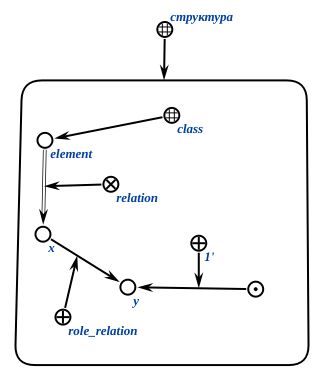
\includegraphics[scale=1]{author/part2/figures/chapter_kb/structure.png}
%	\caption{Представление структуры в SCg}
%	\label{fig:structure_scg}
%\end{figure}

Выделяют следующие классы структур:
\begin{SCn}
	\scnheader{структура}
	\begin{scnrelfromset}{разбиение}
	\scnitem{связная структура}
	\scnitem{несвязная структура}
\end{scnrelfromset}
	\begin{scnrelfromset}{разбиение}
	\scnitem{тривиальная структура}
	\scnitem{нетривиальная структура}
\end{scnrelfromset}
\end{SCn}

\textit{Структуре}, представленной в \textit{SC-коде}, поставим в соответствие орграф, вершинами которого являются \textit{sc-элементы}, а дугами – пары инцидентности, связывающие \textit{sc-коннекторы} с инцидентными им \textit{sc-элементами}, которые являются компонентами указанных \textit{sc-коннекторов}. Если полученный таким способом орграф является связным орграфом, то исходную структуру будем считать \textit{связной структурой}. Если полученный таким способом орграф не является связным орграфом, то исходную структуру будем считать \textit{несвязной структурой}.

Каждая выделяемая структура может выступать в роли либо тривиальной структуры: структуры, которая не содержит связки в качестве элементов, либо в роли нетривиальной структуры: структуры, среди элементов которой есть хотя бы одна связка.

Между структурами можно определять ряд соответствий, таких как гомоморфизм, полиморфизм, автоморфизм, изоморфизм, а также аналогичность структур, что позволяет фиксировать факт наличия некоторой аналогии, сходства и различия некоторых подструктур рассматриваемых структур.

%Пример отношения \textit{аналогичность структур} в SCg представлен на рисунке \textit{\nameref{fig:structure_analogy_scg}}.

%\begin{figure}[H]
%	\centering
%	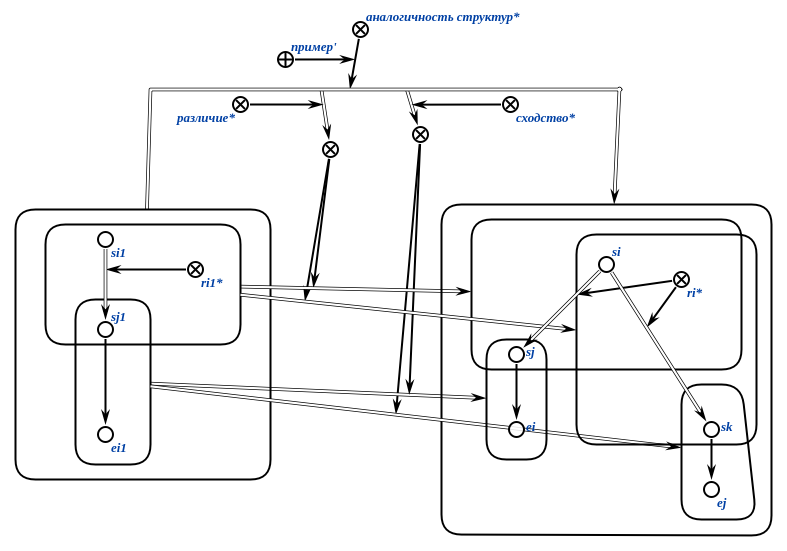
\includegraphics[scale=0.8]{author/part2/figures/chapter_kb/analogy.png}
%	\caption{Пример отношения аналогичность структур в SCg}
%	\label{fig:structure_analogy_scg}
%\end{figure}

\section{Формальная онтология семантических окрестностей}

Для спецификации отдельных сущностей в рамках базы знаний вводиться понятие \textit{семантической окрестности}. Семантическая окрестность представляет собой спецификацию (описание) заданной сущности, знак которой указывается как ключевой элемент этой спецификации.

Набор признаков, по которым можно специфицировать сущности, различен.

Различают полную и базовую семантические окрестности.

\begin{SCn}
	\scnheader{полная семантическая окрестность}
	\scnidtf{полная спецификация некоторой описываемой сущности}
\end{SCn}

Структура \textit{полной семантической окрестности} определяется прежде всего семантической типологией описываемой сущности.
Так, например, для понятия в \textit{полную семантическую окрестность} необходимо включить следующую
информацию (при наличии):
\begin{itemize}
	\item{варианты идентификации на различных внешних языках (sc-идентификаторы)};
	\item{принадлежность некоторой предметной области с указанием роли, выполняемой в рамках этой предметной области};
	\item{теоретико-множественные связи заданного понятия с другими sc-элементами};
	\item{определение или пояснение};
	\item{высказывания, описывающие свойства указанного понятия};
	\item{задачи и их классы, в которых данное понятие является ключевым};
	\item{описание типичного примера использования указанного понятия};
	\item{экземпляры описываемого понятия}.
\end{itemize}

Для понятия, являющегося отношением дополнительно указываются:
\begin{itemize}
	\item {домены};
	\item{область определения};
	\item{схема отношения};
	\item{классы отношений, которым принадлежит описываемое отношение}.
\end{itemize}

\begin{SCn}
	\scnheader{базовая семантическая окрестность}
	\scnidtf{минимально достаточная семантическая окрестность}
	\scnidtf{минимальная спецификация описываемой сущности}
\end{SCn}

Структура \textit{базовой семантической окрестности} определяется прежде всего семантической типологией описываемой сущности. Так, например, для понятия в \textit{базовую семантическую окрестность} необходимо включить следующую  информацию (при наличии):
\begin{itemize}
	\item {варианты идентификации на различных внешних языках (sc-идентификаторы)};
	\item {принадлежность некоторой предметной области с указанием роли, выполняемой в рамках этой предметной области};
	\item{определение или пояснение}.
\end{itemize}

Для понятия, являющегося отношением дополнительно указываются:
\begin{itemize}
	\item {домены};
	\item {область определения};
	\item {описание типичного примера связки указанного отношения (спецификация типичного экземпляра)}.
\end{itemize}

\section{Формальная онтология предметных областей}

Важнейшим этапом разработки баз знаний является процесс выделения описываемых предметных областей и их представления в базе знаний.

Понятие \textit{\textbf{предметной области}} является важнейшим методологическим приемом, позволяющим выделить из всего многообразия исследуемого Мира только определенный класс исследуемых сущностей и только определенное семейство отношений, заданных на указанном классе. То есть осуществляется локализация,
фокусирование внимания только на этом, абстрагируясь от всего остального исследуемого Мира.

Каждой \textit{предметной области} можно поставить в соответствие:
\begin{itemize}
	\item {семейство соответствующих ей онтологий разного вида};
	\item {множество семантических окрестностей, описывающих объекты исследования этой предметной области}.
\end{itemize}


\section{Формальная онтология онтологий}

Для формальной спецификации соответствующей предметной области,
ориентированной на описание свойств и взаимосвязей понятий, входящих в состав указанной предметной области, используется такой вид знаний, как \textit{онтология}.

\begin{SCn}
	\scnheader{онтология}
	\scnidtf{sc-онтология}
	\scnidtf{семантическая спецификация любого знания, имеющего достаточно сложную структуру, любого целостного
		фрагмента базы знаний – предметной области, метода решения сложных задач некоторого класса, описания
		истории некоторого вида деятельности, описания области выполнения некоторого множества действий
		(области решения задач), языка представления методов решения задач и т.д}
\end{SCn}

Онтология включает в себя:
\begin{itemize}
	\item {типологию специфицируемого знания};
	\item{связи специфицируемого знания с другими знаниями};
	\item{спецификацию ключевых понятий, используемых в специфицируемом знании, а также ключевых экземпляров некоторых таких понятий}.
\end{itemize}

Онтологии являются важнейшим видом знаний, обеспечивающих семантическую систематизацию знаний, хранимых в памяти интеллектуальных компьютерных систем (в т.ч. ostis-систем), и, соответственно, семантическую структуризацию баз знаний.

%%%%%%%%%%%%%%%%%%%%%%%%% referenc.tex %%%%%%%%%%%%%%%%%%%%%%%%%%%%%%
% sample references
% %
% Use this file as a template for your own input.
%
%%%%%%%%%%%%%%%%%%%%%%%% Springer-Verlag %%%%%%%%%%%%%%%%%%%%%%%%%%
%
% BibTeX users please use
% \bibliographystyle{}
% \bibliography{}
%
\biblstarthook{In view of the parallel print and (chapter-wise) online publication of your book at \url{www.springerlink.com} it has been decided that -- as a genreral rule --  references should be sorted chapter-wise and placed at the end of the individual chapters. However, upon agreement with your contact at Springer you may list your references in a single seperate chapter at the end of your book. Deactivate the class option \texttt{sectrefs} and the \texttt{thebibliography} environment will be put out as a chapter of its own.\\\indent
References may be \textit{cited} in the text either by number (preferred) or by author/year.\footnote{Make sure that all references from the list are cited in the text. Those not cited should be moved to a separate \textit{Further Reading} section or chapter.} If the citatiion in the text is numbered, the reference list should be arranged in ascending order. If the citation in the text is author/year, the reference list should be \textit{sorted} alphabetically and if there are several works by the same author, the following order should be used:
\begin{enumerate}
\item all works by the author alone, ordered chronologically by year of publication
\item all works by the author with a coauthor, ordered alphabetically by coauthor
\item all works by the author with several coauthors, ordered chronologically by year of publication.
\end{enumerate}
The \textit{styling} of references\footnote{Always use the standard abbreviation of a journal's name according to the ISSN \textit{List of Title Word Abbreviations}, see \url{http://www.issn.org/en/node/344}} depends on the subject of your book:
\begin{itemize}
\item The \textit{two} recommended styles for references in books on \textit{mathematical, physical, statistical and computer sciences} are depicted in ~\cite{science-contrib, science-online, science-mono, science-journal, science-DOI} and ~\cite{phys-online, phys-mono, phys-journal, phys-DOI, phys-contrib}.
\item Examples of the most commonly used reference style in books on \textit{Psychology, Social Sciences} are~\cite{psysoc-mono, psysoc-online,psysoc-journal, psysoc-contrib, psysoc-DOI}.
\item Examples for references in books on \textit{Humanities, Linguistics, Philosophy} are~\cite{humlinphil-journal, humlinphil-contrib, humlinphil-mono, humlinphil-online, humlinphil-DOI}.
\item Examples of the basic Springer style used in publications on a wide range of subjects such as \textit{Computer Science, Economics, Engineering, Geosciences, Life Sciences, Medicine, Biomedicine} are ~\cite{basic-contrib, basic-online, basic-journal, basic-DOI, basic-mono}. 
\end{itemize}
}

\begin{thebibliography}{99.}%
% and use \bibitem to create references.
%
% Use the following syntax and markup for your references if 
% the subject of your book is from the field 
% "Mathematics, Physics, Statistics, Computer Science"
%
% Contribution 
\bibitem{science-contrib} Broy, M.: Software engineering --- from auxiliary to key technologies. In: Broy, M., Dener, E. (eds.) Software Pioneers, pp. 10-13. Springer, Heidelberg (2002)
%
% Online Document
\bibitem{science-online} Dod, J.: Effective substances. In: The Dictionary of Substances and Their Effects. Royal Society of Chemistry (1999) Available via DIALOG. \\
\url{http://www.rsc.org/dose/title of subordinate document. Cited 15 Jan 1999}
%
% Monograph
\bibitem{science-mono} Geddes, K.O., Czapor, S.R., Labahn, G.: Algorithms for Computer Algebra. Kluwer, Boston (1992) 
%
% Journal article
\bibitem{science-journal} Hamburger, C.: Quasimonotonicity, regularity and duality for nonlinear systems of partial differential equations. Ann. Mat. Pura. Appl. \textbf{169}, 321--354 (1995)
%
% Journal article by DOI
\bibitem{science-DOI} Slifka, M.K., Whitton, J.L.: Clinical implications of dysregulated cytokine production. J. Mol. Med. (2000) doi: 10.1007/s001090000086 
%
\bigskip

% Use the following (APS) syntax and markup for your references if 
% the subject of your book is from the field 
% "Mathematics, Physics, Statistics, Computer Science"
%
% Online Document
\bibitem{phys-online} J. Dod, in \textit{The Dictionary of Substances and Their Effects}, Royal Society of Chemistry. (Available via DIALOG, 1999), 
\url{http://www.rsc.org/dose/title of subordinate document. Cited 15 Jan 1999}
%
% Monograph
\bibitem{phys-mono} H. Ibach, H. L\"uth, \textit{Solid-State Physics}, 2nd edn. (Springer, New York, 1996), pp. 45-56 
%
% Journal article
\bibitem{phys-journal} S. Preuss, A. Demchuk Jr., M. Stuke, Appl. Phys. A \textbf{61}
%
% Journal article by DOI
\bibitem{phys-DOI} M.K. Slifka, J.L. Whitton, J. Mol. Med., doi: 10.1007/s001090000086
%
% Contribution 
\bibitem{phys-contrib} S.E. Smith, in \textit{Neuromuscular Junction}, ed. by E. Zaimis. Handbook of Experimental Pharmacology, vol 42 (Springer, Heidelberg, 1976), p. 593
%
\bigskip
%
% Use the following syntax and markup for your references if 
% the subject of your book is from the field 
% "Psychology, Social Sciences"
%
%
% Monograph
\bibitem{psysoc-mono} Calfee, R.~C., \& Valencia, R.~R. (1991). \textit{APA guide to preparing manuscripts for journal publication.} Washington, DC: American Psychological Association.
%
% Online Document
\bibitem{psysoc-online} Dod, J. (1999). Effective substances. In: The dictionary of substances and their effects. Royal Society of Chemistry. Available via DIALOG. \\
\url{http://www.rsc.org/dose/Effective substances.} Cited 15 Jan 1999.
%
% Journal article
\bibitem{psysoc-journal} Harris, M., Karper, E., Stacks, G., Hoffman, D., DeNiro, R., Cruz, P., et al. (2001). Writing labs and the Hollywood connection. \textit{J Film} Writing, 44(3), 213--245.
%
% Contribution 
\bibitem{psysoc-contrib} O'Neil, J.~M., \& Egan, J. (1992). Men's and women's gender role journeys: Metaphor for healing, transition, and transformation. In B.~R. Wainrig (Ed.), \textit{Gender issues across the life cycle} (pp. 107--123). New York: Springer.
%
% Journal article by DOI
\bibitem{psysoc-DOI}Kreger, M., Brindis, C.D., Manuel, D.M., Sassoubre, L. (2007). Lessons learned in systems change initiatives: benchmarks and indicators. \textit{American Journal of Community Psychology}, doi: 10.1007/s10464-007-9108-14.
%
%
% Use the following syntax and markup for your references if 
% the subject of your book is from the field 
% "Humanities, Linguistics, Philosophy"
%
\bigskip
%
% Journal article
\bibitem{humlinphil-journal} Alber John, Daniel C. O'Connell, and Sabine Kowal. 2002. Personal perspective in TV interviews. \textit{Pragmatics} 12:257--271
%
% Contribution 
\bibitem{humlinphil-contrib} Cameron, Deborah. 1997. Theoretical debates in feminist linguistics: Questions of sex and gender. In \textit{Gender and discourse}, ed. Ruth Wodak, 99--119. London: Sage Publications.
%
% Monograph
\bibitem{humlinphil-mono} Cameron, Deborah. 1985. \textit{Feminism and linguistic theory.} New York: St. Martin's Press.
%
% Online Document
\bibitem{humlinphil-online} Dod, Jake. 1999. Effective substances. In: The dictionary of substances and their effects. Royal Society of Chemistry. Available via DIALOG. \\
http://www.rsc.org/dose/title of subordinate document. Cited 15 Jan 1999
%
% Journal article by DOI
\bibitem{humlinphil-DOI} Suleiman, Camelia, Daniel C. O'Connell, and Sabine Kowal. 2002. `If you and I, if we, in this later day, lose that sacred fire...': Perspective in political interviews. \textit{Journal of Psycholinguistic Research}. doi: 10.1023/A:1015592129296.
%
%
%
\bigskip
%
%
% Use the following syntax and markup for your references if 
% the subject of your book is from the field 
% "Computer Science, Economics, Engineering, Geosciences, Life Sciences"
%
%
% Contribution 
\bibitem{basic-contrib} Brown B, Aaron M (2001) The politics of nature. In: Smith J (ed) The rise of modern genomics, 3rd edn. Wiley, New York 
%
% Online Document
\bibitem{basic-online} Dod J (1999) Effective Substances. In: The dictionary of substances and their effects. Royal Society of Chemistry. Available via DIALOG. \\
\url{http://www.rsc.org/dose/title of subordinate document. Cited 15 Jan 1999}
%
% Journal article by DOI
\bibitem{basic-DOI} Slifka MK, Whitton JL (2000) Clinical implications of dysregulated cytokine production. J Mol Med, doi: 10.1007/s001090000086
%
% Journal article
\bibitem{basic-journal} Smith J, Jones M Jr, Houghton L et al (1999) Future of health insurance. N Engl J Med 965:325--329
%
% Monograph
\bibitem{basic-mono} South J, Blass B (2001) The future of modern genomics. Blackwell, London 
%
\end{thebibliography}
